\documentclass{scrreprt}

\usepackage{amsmath}
\usepackage{amsthm}
\usepackage{amssymb}
\usepackage{bm}
\usepackage[shortlabels]{enumitem}
\usepackage{framed}
\usepackage{hyperref}
\usepackage[utf8]{inputenc}
\usepackage{multicol}
\usepackage{mathtools}
\usepackage{physics}
\usepackage{polynom}
\usepackage{tabularx}
\usepackage[table]{xcolor}
\usepackage{titling}
\usepackage{fancyhdr}
\usepackage{xfrac}
\usepackage{pgfplots}

\pgfplotsset{compat = newest}
\usepgfplotslibrary{fillbetween}
\usetikzlibrary{patterns}
\usetikzlibrary{through}


\author{Karsten Lehmann}
\date{WiSe 2024/25}
\title{Übungsblatt 2\\INF-B-110, Lineare Algebra}

\setlength{\headheight}{26pt}
\pagestyle{fancy}
\fancyhf{}
\lhead{\thetitle}
\rhead{\theauthor}
\lfoot{\thedate}
\rfoot{Seite \thepage}

\begin{document}
\paragraph{Ü3.3  Lösen linearer Gleichungssysteme in Zeilenstufenform}
Für zwei lineare Gleichungssysteme $Ax = b$ über $\mathbb{R}$ ist die erweiterte
Koeffizientenmatrix $\qty\big(A{\Big|}b)$ in Zeilenstufenform gegeben.
Ermitteln Sie die jeweiligen Lösungsmengen!

\[
  \text{(i)} \;
  \qty(
  \begin{array}{ccc|c}
    1 & 1  & -1 & 9   \\
    0 & -3 & 1  & -17 \\
    0 & 0  & 0  & -9
  \end{array}
  )
  \qquad
  \text{(ii)} \;
  \qty(
  \begin{array}{cccc|c}
    1 & 1 & -1 & 3   & 4 \\
    0 & 0 & 2  & -10 & 6 \\
    0 & 0 & 0  & 0   & 0
  \end{array})
\]

\subparagraph{Lsg.} Es sind
\begin{enumerate}[(i)]
\item $\mathbb{L} = \emptyset$ (Die 3. Zeile ist nicht lösbar)
\item
  Es sind $b_3 -5 b_4 = 3$ und $b_1 + b_2 -2 b_4 = 7$. Also
  $\mathbb{L} = \qty{\begin{pmatrix}7 - b_2 + 2b_4 \\ b_2 \\ 3 + 5b_4 \\ b_4 \end{pmatrix}
    \;\middle|\; b_2, b_4 \in \mathbb{R}}$
\end{enumerate}

\paragraph{Ü 3.4 Lösung linearer Gleichungssysteme mit Gauß-Jordan}
Lösen Sie die gegebenen linearen Gleichungssysteme über $\mathbb{R}$ mit dem
Gauß-Jordan-Verfahren.
Markieren Sie dabei die Zeilenstufenform und entscheiden Sie die Lösbarkeit.
Bringen Sie die erweiterte Koeffizientenmatrix schließlich in reduzierte
Zeilenstufenform und lesen Sie daraus die Lösungsmenge des ursprünglichen
Gleichungssystemes ab.

\[
  \text{(i)} \;
  \begin{array}{rcrcrcrcc}
    x_1  & + & x_2  & - & x_3 & + & x_4  & = & 8 \\
    2x_1 & + & x_2  & - & x_3 & - & x_4  & = & 3 \\
    x_1  & + & 2x_2 & + & x_3 & - & 2x_4 & = & 0 \\
    x_1  & - & x_2  & - & x_3 & + & 3x_4 & = & 12 \\
  \end{array}
  \qquad
  \text{(ii)} \;
  \begin{array}{rcrcrcc}
    x_1  & + & 2x_2 & + & x_3  & = & 0 \\
    x_1  & + & x_2  & + & 3x_3 & = & 0 \\
    -x_1 & + & 4x_2 & + & 3x_3 & = & 0 \\
  \end{array}
\]
\subparagraph{Lsg.} Es sind
\begin{enumerate}[(i)]
\item
  \begin{small}
    \begin{flalign*}
      \qty(\begin{array}{cccc|c}
        1 & 1  & -1 & 1  & 8  \\
        2 & 1  & -1 & -1 & 3  \\
        1 & 2  & 1  & -2 & 0  \\
        1 & -1 & -1 & 3  & 12 \\
      \end{array})
      &\overset{Z_2 - 2 \cdot Z_3}\leadsto
      \qty(\begin{array}{cccc|c}
        1 & 1  & -1 & 1  & 8  \\
        0 & -3 & -3 & 3  & 3  \\
        1 & 2  & 1  & -2 & 0  \\
        1 & -1 & -1 & 3  & 12 \\
      \end{array})
      \overset{Z_3 - Z_4}\leadsto
      \qty(\begin{array}{cccc|c}
        1 & 1  & -1 & 1  & 8   \\
        0 & -3 & -3 & 3  & 3   \\
        0 & 3  & 2  & -5 & -12 \\
        1 & -1 & -1 & 3  & 12  \\
      \end{array}) & \\
       \overset{Z_4 - Z_1}\leadsto
      \qty(\begin{array}{cccc|c}
        1 & 1  & -1 & 1  & 8   \\
        0 & -3 & -3 & 3  & 3   \\
        0 & 3  & 2  & -5 & -12 \\
        0 & -2 & 0  & 2  & 4   \\
      \end{array})
      &\overset{Z_3 + Z_2}\leadsto
      \qty(\begin{array}{cccc|c}
        1 & 1  & -1 & 1  & 8  \\
        0 & -3 & -3 & 3  & 3  \\
        0 & 0  & -1 & -2 & -9 \\
        0 & -2 & 0  & 2  & 4  \\
      \end{array})
      \overset{3 \cdot Z_4 - 2 \cdot Z_2}\leadsto
      \qty(\begin{array}{cccc|c}
        1 & 1  & -1 & 1  & 8  \\
        0 & -3 & -3 & 3  & 3  \\
        0 & 0  & -1 & -2 & -9 \\
        0 & 0  & 6  & 0  & 6  \\
      \end{array}) \\
      \overset{Z_4 \leftrightarrow Z_3}\leadsto
      \qty(\begin{array}{cccc|c}
        1 & 1  & -1 & 1  & 8  \\
        0 & -3 & -3 & 3  & 3  \\
        0 & 0  & 6  & 0  & 6  \\
        0 & 0  & -1 & -2 & -9 \\
      \end{array})
      &\overset{6 \cdot Z_4 + Z_3}\leadsto
      \qty(\begin{array}{cccc|c}
        1 & 1  & -1 & 1   & 8   \\
        \cline{1-1}
        0 & \multicolumn{1}{|c}{-3} & -3 & 3   & 3   \\
        \cline{2-2}
        0 & 0  & \multicolumn{1}{|c}{6} & 0 & 6 \\
        \cline{3-3}
        0 & 0  & 0  & \multicolumn{1}{|c|}{-12} & -48 \\
      \end{array})
    \end{flalign*}
  \end{small}

  \newpage
  $\Rightarrow$ das LGS ist lösbar mit
  \begin{small}
    \begin{flalign*}
      \qty(\begin{array}{cccc|c}
          1 & 1  & -1 & 1   & 8   \\
          0 & -3 & -3 & 3   & 3   \\
          0 & 0  & 6  & 0   & 6   \\
          0 & 0  & 0  & -12 & -48 \\
        \end{array})
      &\overset{-\frac{1}{12} \cdot Z_4}\leadsto
      \qty(\begin{array}{cccc|c}
          1 & 1  & -1 & 1 & 8 \\
          0 & -3 & -3 & 3 & 3 \\
          0 & 0  & 6  & 0 & 6 \\
          0 & 0  & 0  & 1 & 4 \\
        \end{array})
      \overset{\frac{1}{6} \cdot Z_3}\leadsto
      \qty(\begin{array}{cccc|c}
          1 & 1  & -1 & 1 & 8 \\
          0 & -3 & -3 & 3 & 3 \\
          0 & 0  & 1  & 0 & 1 \\
          0 & 0  & 0  & 1 & 4 \\
      \end{array}) \\
      \overset{Z_2 + 3 \cdot Z_3 - 3 \cdot Z_4}\leadsto
      \qty(\begin{array}{cccc|c}
          1 & 1  & -1 & 1 & 8  \\
          0 & -3 & 0  & 0 & -6 \\
          0 & 0  & 1  & 0 & 1  \\
          0 & 0  & 0  & 1 & 4  \\
      \end{array})
      &\overset{-\frac{1}{3} \cdot Z_2}\leadsto
      \qty(\begin{array}{cccc|c}
          1 & 1 & -1 & 1 & 8 \\
          0 & 1 & 0  & 0 & 2 \\
          0 & 0 & 1  & 0 & 1 \\
          0 & 0 & 0  & 1 & 4 \\
      \end{array})
      \overset{Z_1 - Z_2 + Z_3 - Z_4}\leadsto
      \qty(\begin{array}{cccc|c}
          1 & 0 & 0 & 0 & 3 \\
          0 & 1 & 0 & 0 & 2 \\
          0 & 0 & 1 & 0 & 1 \\
          0 & 0 & 0 & 1 & 4 \\
      \end{array})
    \end{flalign*}
    $\Rightarrow \mathbb{L} = \qty{\begin{pmatrix}3 \\ 2 \\ 1 \\ 4\end{pmatrix}}$
  \end{small}

\item
  \begin{small}
    \begin{flalign*}
      \qty(\begin{array}{ccc|c}
        1  & 2  & 1 & 0 \\
        1  & 1  & 3 & 0 \\
        -1 & -4 & 3 & 0 \\
      \end{array})
      &\overset{Z_2 + Z_3}\leadsto
      \qty(\begin{array}{ccc|c}
        1  & 2  & 1 & 0 \\
        0  & -3 & 6 & 0 \\
        -1 & -4 & 3 & 0 \\
      \end{array})
      \overset{Z_3 + Z_1}\leadsto
      \qty(\begin{array}{ccc|c}
        1 & 2  & 1 & 0 \\
        0 & -3 & 6 & 0 \\
        0 & -2 & 4 & 0 \\
      \end{array}) \\
      \overset{3 \cdot Z_3 - 2 \cdot Z_2}\leadsto
      \qty(\begin{array}{ccc|c}
        1 & 2  & 1 & 0 \\
        \cline{1-1}
        0 & \multicolumn{1}{|c}{-3} & 6 & 0 \\
        \cline{2-3}
        0 & 0  & 0 & 0 \\
      \end{array})
    \end{flalign*}
  \end{small}
  $\Rightarrow$ das LGS hat unendlich viele Lösungen mit
  \begin{small}
    \begin{flalign*}
      \qty(\begin{array}{ccc|c}
        1 & 2  & 1 & 0 \\
        0 & -3 & 6 & 0 \\
        0 & 0  & 0 & 0 \\
      \end{array})
      &\overset{-\frac{1}{3}Z_2}\leadsto
      \qty(\begin{array}{ccc|c}
        1 & 2 & 1  & 0 \\
        0 & 1 & -2 & 0 \\
        0 & 0 & 0  & 0 \\
      \end{array})
      \overset{Z_1 - 2 \cdot Z_2}\leadsto
      \qty(\begin{array}{ccc|c}
        1 & 0 & 5  & 0 \\
        0 & 1 & -2 & 0 \\
        0 & 0 & 0  & 0 \\
      \end{array})
    \end{flalign*}
    $\Rightarrow \mathbb{L} = \qty{\begin{pmatrix}-5 \cdot x \\ 2 \cdot x \\ x \end{pmatrix}
    \:\middle|\: x \in \mathbb{R}}$
  \end{small}
\end{enumerate}

\newpage
\paragraph{Ü 3.5 Modellierung mit Linearen Gleichungssystemen}
Ermitteln Sie die Verkehrsströme in den einzelnen Teilstücken des angegebenen
Streckennetzes.
Stellen Sie dazu ein lineares Gleichungssystem auf und berechnen Sie die
Lösungsmenge.
Geben Sie für die Teilstücke $x_2, x_3, x_4$ jeweils die minimale nichtnegative
Lösung an.

\begin{tikzpicture}
  \node[circle, draw] (k1) at (0, 0) {$k_1$};
  \node[circle, draw] (k2) at (4, 0) {$k_2$};
  \node[circle, draw] (k3) at (2, -2) {$k_3$};
  \node[circle, draw] (k4) at (0, -4) {$k_4$};
  \node[circle, draw] (k5) at (4, -4) {$k_5$};

  \draw[->, line width=1mm] (0, 1.5) -- node [right] {30} (k1);
  \draw[->, line width=1mm] (k1) -- node [above] {80} (-1.5, 0);
  \draw[->, line width=1mm] (k1) -- node [left] {$x_1$} (k4);
  \draw[->, line width=1mm] (k2) -- node [left] {$x_5$} (k3);
  \draw[->, line width=1mm] (k4) -- node [right] {$x_3$} (k3);
  \draw[->, line width=1mm] (k3) -- node [left] {$x_2$} (k1);
  \draw[->, line width=1mm] (k3) -- node [right] {$x_4$} (k5);
  \draw[->, line width=1mm] (k5) -- node [right] {$x_6$} (k2);
  \draw[->, line width=1mm] (k2) -- node [right] {40} (4, 1.5);
  \draw[->, line width=1mm] (k4) -- node [right] {20} (0, -5.5);
  \draw[->, line width=1mm] (k5) -- node [above] {90} (5.5, -4);
  \draw[->, line width=1mm] (5.5, 0) -- node [above] {100} (k2);
  \draw[->, line width=1mm] (4, -5.5) -- node [right] {40} (k5);
  \draw[->, line width=1mm] (-1.5, -4) -- node [above] {60} (k4);
\end{tikzpicture}

\subparagraph{Lsg.} Am Knoten $k_1$ gehen 30 und $x_2$ ein, sowie 80 und $x_1$ aus.
Es folgt
\[
  30 + x_2 = 80 + x_1
\]
Am Knoten $k_2$ gehen 100 und $x_6$ ein, sowie 40 und $x_5$ aus.
Es folgt
\[
  100 + x_6 = 40 + x_5
\]
Am Knoten $k_3$ gehen $x_3$ und $x_5$ ein, sowie $x_2$ und $x_4$ aus.
Es folgt
\[
  x_3 + x_5 = x_2 + x_4
\]
Am Knoten $k_4$ gehen $x_1$ und 60 ein, sowie $x_3$ und 20 aus.
Es folgt
\[
  x_1 + 60 = x_3 + 20
\]
Am Knoten $k_5$ gehen $x_4$ und 40 ein, sowie $x_6$ und 90 aus.
Es folgt
\[
  x_4 + 40 = x_6 + 90
\]

Somit ergibt sich ein LGS mit 5 Gleichungen und 6 Unbekannten:
\begin{flalign*}
  \qty(\begin{array}{cccccc|c}
    1  & -1 & 0  & 0 & 0  & 0  & -50 \\
    0  & 1  & -1 & 1 & -1 & 0  & 0   \\
    -1 & 0  & 1  & 0 & 0  & 0  & 40  \\
    0  & 0  & 0  & 1 & 0  & -1 & 50  \\
    0  & 0  & 0  & 0 & 1  & -1 & 60  \\
  \end{array})
  &\overset{Z_3 + Z_2 + Z_1}\leadsto
  \qty(\begin{array}{cccccc|c}
    1 & -1 & 0  & 0 & 0  & 0  & -50 \\
    0 & 1  & -1 & 1 & -1 & 0  & 0   \\
    0 & 0  & 0  & 1 & -1 & 0  & -10 \\
    0 & 0  & 0  & 1 & 0  & -1 & 50  \\
    0 & 0  & 0  & 0 & 1  & -1 & 60  \\
  \end{array}) \\
  &\overset{Z_4 - Z_3}\leadsto
  \qty(\begin{array}{cccccc|c}
    1 & -1 & 0  & 0 & 0  & 0  & -50 \\
    0 & 1  & -1 & 1 & -1 & 0  & 0   \\
    0 & 0  & 0  & 1 & -1 & 0  & -10 \\
    0 & 0  & 0  & 0 & 1  & -1 & 60  \\
    0 & 0  & 0  & 0 & 1  & -1 & 60  \\
  \end{array})
\end{flalign*}

Es bleiben die Gleichungen
\begin{flalign*}
  x_1 - x_2 = -50 &\Rightarrow x_1 = x_2 - 50 \\
  x_4 - x_5 = -10 &\Rightarrow x_4 = x_5 - 10 \\
  x_5 - x_6 = 60 &\Rightarrow x_6 = x_5 - 60 \\
  x_2 - x_3 + x_4 - x_5 = 0 &\Rightarrow x_3 = x_2 + x_4 - x_5 = x_2 - \qty\big(x_5 - 10) - x_5 = x_2 - 10
\end{flalign*}

\[
  \mathbb{L} = \qty{
    \begin{pmatrix}
      x_2 - 50 \\
      x_2 \\
      x_2 - 10 \\
      x_5 - 10 \\
      x_5 \\
      x_5 - 60 \\
    \end{pmatrix}
    \:\middle|\:
    x_2, x_4, x_5 \in \mathbb{N}
  }
\]

Unter der Annahme, dass der Lösungsvektor in $\mathbb{N}^6$ liegt, folgen
\begin{itemize}
\item $x_1 \geq 0$
\item $x_2 \geq 50$
\item $x_3 \geq 40$
\item $x_4 \geq 50$
\item $x_5 \geq 60$
\item $x_6 \geq 0$
\end{itemize}

\newpage
\paragraph{Ü 3.6 Lineares Gleichungssystem über $\text{GF}(2)$}

Bestimmen Sie die Lösungsmenge des folgenden linearen Gleichungssystems über
GF(2):
\[
  \begin{pmatrix}
    1 & 1 & 1 & 0 & 1 & 0 & 0 \\
    1 & 1 & 0 & 1 & 0 & 1 & 0 \\
    1 & 0 & 1 & 1 & 0 & 0 & 1 \\
  \end{pmatrix}
  \cdot
  \begin{pmatrix}
    x_1 \\
    x_2 \\
    x_3 \\
    x_4 \\
    x_5 \\
    x_6 \\
    x_7 \\
  \end{pmatrix}
  =
  \begin{pmatrix}
    0 \\
    0 \\
    0 \\
  \end{pmatrix}
\]
Wie viele Elemente hat die Lösungsmenge?

\subparagraph{Lsg.} Es ist
\begin{flalign*}
  \qty(\begin{array}{ccccccc|c}
    1 & 1 & 1 & 0 & 1 & 0 & 0 & 0 \\
    1 & 1 & 0 & 1 & 0 & 1 & 0 & 0 \\
    1 & 0 & 1 & 1 & 0 & 0 & 1 & 0 \\
  \end{array})
  &\overset{Z_2 + Z_3}\leadsto
  \qty(\begin{array}{ccccccc|c}
    1 & 1 & 1 & 0 & 1 & 0 & 0 & 0 \\
    0 & 1 & 1 & 0 & 0 & 1 & 1 & 0 \\
    1 & 0 & 1 & 1 & 0 & 0 & 1 & 0 \\
  \end{array}) & \\
  &\overset{Z_3 + Z_1}\leadsto
  \qty(\begin{array}{ccccccc|c}
    1 & 1 & 1 & 0 & 1 & 0 & 0 & 0 \\
    0 & 1 & 1 & 0 & 0 & 1 & 1 & 0 \\
    0 & 1 & 0 & 1 & 1 & 0 & 1 & 0 \\
  \end{array}) & \\
  &\overset{Z_3 + Z_2}\leadsto
  \qty(\begin{array}{ccccccc|c}
    1 & 1 & 1 & 0 & 1 & 0 & 0 & 0 \\
    0 & 1 & 1 & 0 & 0 & 1 & 1 & 0 \\
    0 & 0 & 1 & 1 & 1 & 1 & 0 & 0 \\
  \end{array}) \\
  &\overset{Z_1 - Z_2}\leadsto
  \qty(\begin{array}{ccccccc|c}
    1 & 0 & 0 & 0 & 1 & 1 & 1 & 0 \\
    0 & 1 & 1 & 0 & 0 & 1 & 1 & 0 \\
    0 & 0 & 1 & 1 & 1 & 1 & 0 & 0 \\
  \end{array}) \\
  &\overset{Z_2 - Z_3}\leadsto
  \qty(\begin{array}{ccccccc|c}
    1 & 0 & 0 & 0 & 1 & 1 & 1 & 0 \\
    0 & 1 & 0 & 1 & 1 & 0 & 1 & 0 \\
    0 & 0 & 1 & 1 & 1 & 1 & 0 & 0 \\
  \end{array})
\end{flalign*}
Es folgen die Gleichungen
\begin{flalign*}
  x_1 + x_5 + x_6 + x_7 &= 0 & \\
  x_2 + x_4 + x_5 + x_7 &= 0 \\
  x_3 + x_4 + x_5 + x_6 &= 0
\end{flalign*}
Somit ist
\[
  \mathbb{L} = \qty{
    \begin{pmatrix}
      x_5 + x_6 + x_7 \\
      x_4 + x_5 + x_7 \\
      x_4 + x_5 + x_6 \\
      x_4 \\
      x_5 \\
      x_6 \\
      x_7 \\
    \end{pmatrix}
    \:\middle|\:
    x_4, x_5, x_6, x_7 \in \text{GF}\qty\big(2)
  }
\]
Mit 4 Unbekannten in GF$\qty\big(2)$ folgen $2^4 = 16$ Lösungen.
\end{document}
